\begin{abstract}
Scientific query alternatives share the same missing observations, so independent identification intervals can admit impossible disagreements. We present \CLARA{}, a dependence-aware execution guard for cancer-genomics curation. Patient-block completion tables preserve patient aggregation and nested mutation classes, giving attainable discrepancy witnesses and exact strict-threshold decisions without enumerating global worlds. A violating-pair graph governs clarification; a separate identification guard governs numerical answers. In a frozen 12-cohort, 30-gene TCGA registry, two counting engines agree on all 5,760 specifications. Shared-completion certificates remove 3,048 interval-box alarms among 43,200 pairs, including 289 remaining after exact equivalence merging. Under uniform supported intents, expected clarification is 1.773 questions versus 1.833 for the equivalence-merged baseline, a 3.28\% reduction; the best per-family fixed order matches the dynamic program. A separate MSK-IMPACT cohort adds 480 verified specifications and repeated-specimen counting evidence. However, 720 TCGA specifications lack a point answer within 2.5 percentage points. Serial scaling measurements and a replayable typed interface connect these certificates to curation pipelines. Claims concern supplied interpretations and an explicit assay-record completion model, without human or language-model evaluation.
\end{abstract}
\begin{IEEEkeywords}
scientific data curation, query ambiguity, incomplete databases, cancer genomics, robust optimization, clarification
\end{IEEEkeywords}

\section{Introduction}
``What fraction of kidney cancers have a VHL mutation?'' does not specify an executable estimand. A patient with multiple specimens can contribute once or repeatedly; the denominator can include only assay-eligible units or the full study cohort; specimens can be restricted to primary tumors; and the mutation class set can include missense events or only selected restricted classes. An execution can be syntactically valid while answering a different scientific question.

There is also an observational problem. In the frozen KIRC snapshot, 166 of 402 profiled patients have a recorded VHL broad-class event. The corresponding recorded-positive cohort fraction is 166/512. The 110 unprofiled patients could change the latter target to any feasible value between 32.42\% and 53.91\% in our completion model. Clarifying the denominator does not measure those patients. Conversely, because this cohort has one specimen per patient, patient and specimen queries have identical values in every completion. Comparing the lower endpoint of one interval to the upper endpoint of the other falsely suggests a 21.48-percentage-point (pp) unit discrepancy.

This distinction matters when curation systems decide whether a query needs clarification. Modern systems generate interpretations, ask interactive questions, or guide clarification using uncertainty \cite{nalir,ambiqt,saparina,intentsim,sage}. We address a subsequent execution layer: given a finite set of typed scientific specifications, which differences could matter numerically, and which field questions suffice to resolve them? A result-aware audit should share missing observations across specifications, preserve dependence introduced by patient aggregation and nested mutation classes, and identify when a stable interpretation still lacks a defensible point answer.

\CLARA{} contributes three application-specific components. First, a patient-block representation gives sharp paired discrepancies under a declared assay-record completion model, including partially observed patients. Second, exact count-support decisions build a violating-pair graph, on which expected-cost and minimax planning use classical decision-tree recurrences. Third, a fully retained public-data registry compares observed-only, independent-interval, equivalence-merged interval, and shared-completion certificates. The strongest empirical finding concerns \emph{dependence-aware certification}, not universal superiority of adaptive questioning: the best per-family fixed order matches the optimal planner under the primary uniform scenario.

Possible-world semantics \cite{incomplete} supplies the interpretation of incomplete observations; fractional programming \cite{dinkelbach} converts relative discrepancies into support problems; and optimal identification procedures \cite{garey} motivate cost-aware field selection. We combine these foundations in an executable audit for genomic count queries, with shared patient-level completions, attainable discrepancy witnesses, exact strict-threshold decisions, and a separate numerical-identification guard.

The workshop-relevant scale is computational: KIRC's 110 unknown specimen states induce $3^{110}$ worlds, while the audit visits only 330 local states per gene. The observed registry is small; this is a contextualization and validation layer, rather than an extreme-volume ingestion system. A typed agent can carry the certificate as result metadata, request a relevant field, or return an interval when a point remains unidentified. We measure serial scaling and provide hash-bound replay to make that integration concrete.

\begin{figure*}[t]
\centering
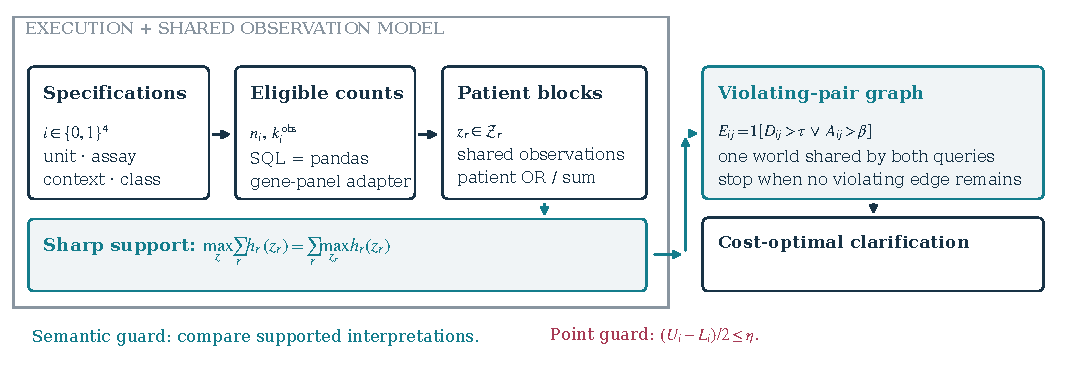
\includegraphics[width=\textwidth]{01_method.pdf}
\caption{The audit separates typed scientific meaning from missing observations. Every alternative shares the same specimen states. Patient-block support produces a violating-pair graph; clarification filters its vertices. A separate identification guard governs whether a point answer is supported. The gene-panel adapter is a schema contract, not evidence of per-base assay coverage.}
\label{fig:method}
\end{figure*}

\section{Related Work}
Partial identification separates what observations determine from what additional assumptions supply \cite{manski}. Our endpoints instantiate this principle for a fixed finite cohort; they are neither population confidence intervals nor causal-effect bounds. Incomplete-database possible worlds \cite{incomplete} and numerical aggregate answers \cite{console} address uncertain query outputs. Console \emph{et al.}\ use distributions over numerical nulls; we instead optimize discrepancies between query functions over shared, nonprobabilistic event states.

Why/where provenance \cite{buneman}, uncertainty with lineage \cite{uldb}, and provenance semirings \cite{green} explain why results derived from shared inputs require linked uncertainty. Our contribution is an executable specialization to genomic counting and two answer guards. The exported receipt records query-level derivation using basic PROV-O entity/activity relations \cite{prov}; it does not compute tuple-level provenance polynomials. Interactive semantic parsing and LLM clarification \cite{nalir,ambiqt,saparina,intentsim,sage} concern identifying intent. We assume the supported candidates are supplied and evaluate their execution consequences, keeping the classical optimization principles explicit.

\section{Scientific Specifications and Shared Completions}
\subsection{Running example: one shared unknown}
Consider two patients and three primary specimens: patient 1 has one recorded-negative specimen and one unprofiled specimen; patient 2 has one recorded-positive specimen. Let $u\in\{0,1\}$ indicate a broad event in the unprofiled specimen. The cohort patient fraction is $(1+u)/2$; the cohort specimen fraction is $(1+u)/3$. The feasible pairs are $(1/2,1/3)$ and $(1,2/3)$, so their largest difference is $1/3$. Independent intervals allow the impossible pair $(1,1/3)$ and double that bound to $2/3$. The shared unknown is the same input to both counting rules.

\subsection{Four fields define an executable family}
For a fixed cohort and gene, the supported family is
\begin{equation}
\mathcal I=\{P,S\}\!\times\!\{E,C\}\!\times\!\{A,R\}\!\times\!\{B,T\},\qquad |\mathcal I|=16,
\label{eq:family}
\end{equation}
where $P/S$ selects patient/specimen units, $E/C$ selects profiled/full-cohort denominators, $A/R$ selects all/primary specimens, and $B/T$ selects broad/restricted consequence classes. The broad set has nine recorded consequence labels; the restricted set has six and is a subset of the broad set. The restricted set includes translation-start-site and nonstop labels; it is not a literal protein-truncating-variant set. We retain the legacy code token \texttt{truncating} for this unchanged operational filter. Neither set establishes pathogenicity or functional loss. Gene, cancer type, other variants, and unsupported interpretations remain outside this lattice.

Indices $i,j$ name specifications, $r$ patients, $s$ specimens, and $q$ question fields throughout.

Let $S_r$ be the specimens of patient $r$, $A_i$ the context-eligible specimens, and $E$ the mutation-profile membership set. In profiled mode the eligible specimen set is $H_i=A_i\cap E$; in cohort mode it is $H_i=A_i$. The fixed denominator $n_i$ is either $|H_i|$ or the number of patients represented in $H_i$. In the observed execution, positive specimens must belong to $A_i\cap E$ before projecting to the chosen counting unit. Zero denominators yield undefined results and cannot receive a certificate.

The profiled fraction is conditional on assay eligibility. A cohort-mode recorded-positive fraction is a lower bound for the completed cohort target, not an unbiased estimate of the same profiled target. Profile membership does not establish gene-level technical sensitivity, coverage at each base, or absence of an unrecorded event \cite{cbio_docs}.

\subsection{One world is shared by all alternatives}
For each unprofiled specimen $s$, let
\begin{equation}
 z_s\in\{0,1,2\},\qquad b_s=\mathbf1[z_s\geq1],\quad t_s=\mathbf1[z_s=2].
\label{eq:latent}
\end{equation}
States denote absent, broad-only, or restricted-and-broad events. Profiled event labels remain fixed at the recorded class-set events. Thus $t_s\leq b_s$ in every completion. This is an \emph{assay-record completion model}; it does not model sequencing errors, pathogenicity, or population prevalence. No probabilistic prior is imposed on missing statuses.

In cohort mode, specimen counts add all context-eligible completed positives. Patient counts take an OR over that patient's eligible specimens, including unprofiled specimens even when another specimen was profiled. Profiled mode uses only profiled specimens. For patient block $r$, let $m_r$ be its unprofiled specimen count, $\mathcal Z_r=\{0,1,2\}^{m_r}$, and $k_{ir}(z_r)$ its positive-unit contribution. After separating fully observed contributions $k_i^0$,
\begin{equation}
 \begin{aligned}
 f_i(z)&=\frac{k_i^0+\sum_r k_{ir}(z_r)}{n_i},\\
 \mathcal Z&=\prod_r\mathcal Z_r.
 \end{aligned}
\label{eq:additive}
\end{equation}
The nonlinear patient OR remains \emph{inside} a local block; the global sum is separable. A repeated-specimen patient need not be treated as independent specimens. For a single fixed specification, the sharp identification endpoints are
\begin{equation}
 \begin{aligned}
 L_i&=\frac{k_i^0+\sum_r\min_{z_r}k_{ir}(z_r)}{n_i},\\
 U_i&=\frac{k_i^0+\sum_r\max_{z_r}k_{ir}(z_r)}{n_i}.
 \end{aligned}
\label{eq:bounds}
\end{equation}
These are possible-value bounds, not confidence intervals. Their sharpness assumes the Cartesian completion space in (\ref{eq:additive}); cross-patient constraints or external biological information would change the model.

\section{Sharp Certificates and Two Answer Guards}
\subsection{Paired absolute discrepancy}
The independent interval box $[L_i,U_i]\times[L_j,U_j]$ contains the joint feasible set, but can be much larger (Fig.~\ref{fig:geometry}). Define
\begin{equation}
 A_{ij}=100\max_{z\in\mathcal Z}|f_i(z)-f_j(z)|.
\end{equation}
\begin{proposition}[Patient-block support]
For arbitrary real $a,b$, write $v_{ir}=k_{ir}/n_i$ and $c_i=k_i^0/n_i$. Then
\begin{equation}
 \begin{aligned}
 H_{ij}(a,b)&=\max_z(af_i(z)+bf_j(z))\\
 &=ac_i+bc_j+\sum_r\max_{z_r}(av_{ir}+bv_{jr}).
 \end{aligned}
\label{eq:support}
\end{equation}
Consequently $A_{ij}=100\max\{H_{ij}(1,-1),H_{ji}(1,-1)\}$, and each maximum has a realizable completion witness.
\end{proposition}
\begin{proof}
Any completion is bounded above by the sum of its local maxima. Select a maximizing state independently in every finite patient block. Their product is feasible and attains that bound. Apply this identity to both directed differences.
\end{proof}
Computing all $K^2$ paired supports costs $O(K^2\sum_r3^{m_r})$, rather than $O(K^2 3^{\sum_r m_r})$. We group identical local contribution tables for computational reuse without altering their multiplicity or statistical interpretation. For KIRC, 110 missing specimens imply $3^{110}$ global worlds but only 330 local states per gene. The implementation refuses blocks above a declared 100,000-state budget; no hidden pruning is used.

\begin{figure*}[t]
\centering
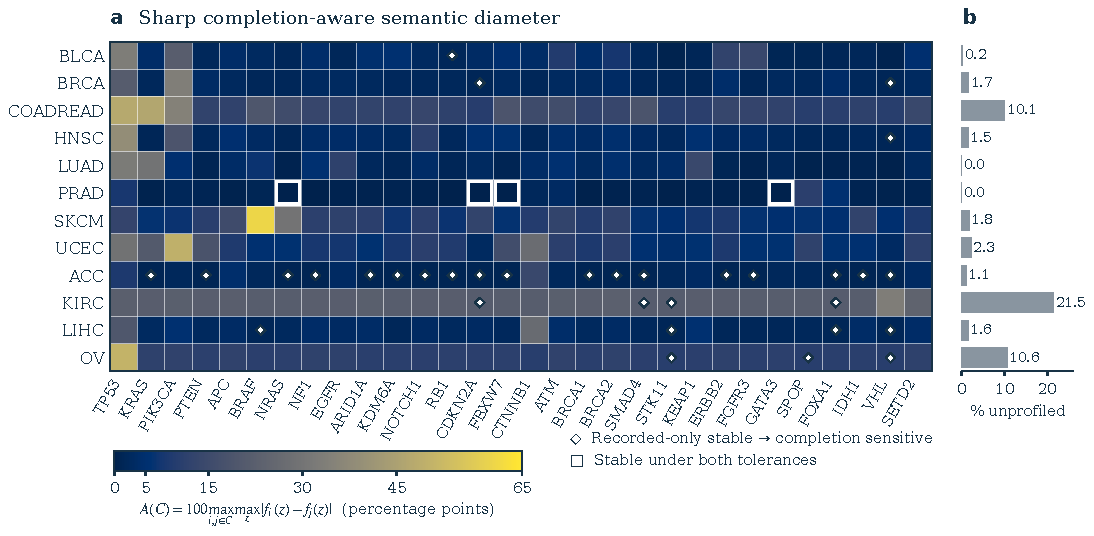
\includegraphics[width=\textwidth]{02_matrix.pdf}
\caption{The retained 12-cohort $\times$ 30-gene matrix. Color gives the sharp absolute semantic diameter over all 16 specifications and all shared completions. Diamonds mark the 33 families stable under recorded counts but sensitive under the completion model; outlined cells mark the four robustly stable families. Classification uses 10\% relative OR 5 pp absolute discrepancy, so color alone does not determine sensitivity. The sidebar gives specimen-level mutation-profile missingness in the all-specimen context. Every family, including zero-event families, is retained.}
\label{fig:matrix}
\end{figure*}

\subsection{Relative discrepancy through parametric support}
For nonnegative fractions and $\epsilon=10^{-12}$, define
\begin{equation}
 D_{ij}=\max_z\frac{|f_i(z)-f_j(z)|}{(f_i(z)+f_j(z))/2+\epsilon}.
\label{eq:relative}
\end{equation}
Applying the standard fractional-to-parametric relation \cite{dinkelbach}, let
\begin{equation}
 \Phi_{ij}(\rho)=H_{ij}(1-\rho/2,-1-\rho/2)-\rho\epsilon.
\label{eq:phi}
\end{equation}
\begin{proposition}[Directional relative support]
If $H_{ij}(1,-1)>0$, the positive directed ratio maximum is the unique root of $\Phi_{ij}(\rho)=0$ in $(0,2)$. Otherwise its positive part is zero. Taking the larger positive part of the two directions gives $D_{ij}$.
\end{proposition}
\begin{proof}
The denominator is strictly positive. For any $\rho$, $\Phi_{ij}(\rho)>0$ exactly when a feasible directed ratio exceeds $\rho$. The maximum of finitely many affine functions is continuous. All slopes are at most $-\epsilon$, so it is strictly decreasing; its sign changes at the largest feasible positive ratio. The reverse direction handles the absolute value.
\end{proof}
Forty bisection iterations produce numerical brackets of nominal width at most $2/2^{40}=1.82\times10^{-12}$. We use them for reporting, \emph{not} primary classification. Threshold labels use integer support and rational comparisons, avoiding floating-point disagreement at a strict cutoff.

For relative threshold $\tau=a/b$, let $M_{ij}$ be the maximum over completions of
\begin{equation}
 (2b-a)k_i(z)n_j-(2b+a)k_j(z)n_i,
\label{eq:integer}
\end{equation}
computed by local integer maxima. Then a directed violation occurs iff $M_{ij}>2a\epsilon n_i n_j$. At $\tau=1/10$, the coefficients are $19$ and $-21$. Likewise, a 5 pp absolute violation occurs iff the largest directed absolute count support satisfies $20M_{ij}^{\rm abs}>n_i n_j$. Counts in the evaluated registries fit signed 64-bit support arithmetic; the final rational comparison is exact. Equality is accepted by the declared strict rule.

\subsection{Semantic stability is a graph property}
Set the primary tolerances to $\tau=0.10$, $\beta=5$ pp. The violating-pair graph has vertices $\mathcal I$ and edges
\begin{equation}
 (i,j)\in E_G\iff D_{ij}>\tau\ \lor\ A_{ij}>\beta.
\label{eq:edge}
\end{equation}
A surviving candidate set $C$ is semantically stable iff $G[C]$ has no edge. This is a conditional certificate: every supported pair lies within both tolerances in every feasible \emph{shared} world. Filtering candidates preserves stability because it deletes vertices. A reference-centered one-axis audit is insufficient: it tests four of the 120 pairs and can miss interacting choices.

\subsection{Point identification is a separate requirement}
At a stable node, an interval answer can report the envelope
\begin{equation}
 [L(C),U(C)]=[\min_{i\in C}L_i,\max_{i\in C}U_i].
\end{equation}
For a worst-case point-error budget $\eta$, the second guard is
\begin{equation}
 R^*(C)=\min_x\max_{i\in C,z}|x-f_i(z)|
 =\frac{U(C)-L(C)}{2}\leq\eta.
\label{eq:guard}
\end{equation}
The midpoint attains this minimax error; it is not an unbiased prevalence estimator. In particular, a singleton has no semantic edge but may fail the point guard. If its interval exceeds $2\eta$, further intent clarification cannot recover missing measurements for that fixed estimand. The system should return the identification interval or request additional evidence. A lower question count must not be interpreted as increased point-answer availability.

\begin{figure*}[t]
\centering
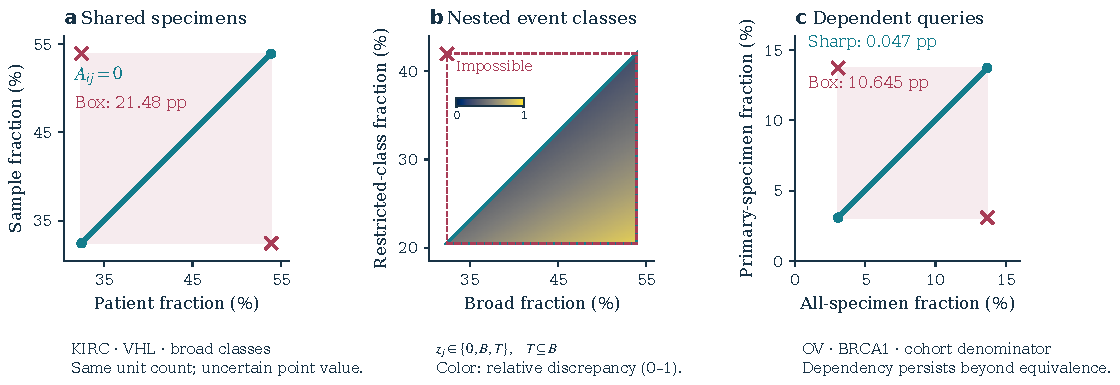
\includegraphics[width=\textwidth]{03_geometry.pdf}
\caption{Dependence in real frozen-snapshot examples. (a) KIRC--VHL patient and specimen cohort queries coincide in every world; their marginal intervals are wide. Red crosses combine incompatible worlds. (b) Broad and restricted KIRC--VHL events occupy a triangular convex hull because the same unprofiled specimen cannot be restricted without being broad; color is relative discrepancy. (c) OV--BRCA1 all-versus-primary cohort queries are distinct but share the same missing events. Their sharp absolute discrepancy is 0.0469 pp, while the independent box permits 10.6452 pp. Lines/regions represent feasible completions or their convex hull, not new patient measurements.}
\label{fig:geometry}
\end{figure*}

\section{Cost-Aware Clarification}
A truthful answer to field $q$ partitions $C$ into $C_{qv}$. Let $w_i>0$ be stipulated intent weights, $w(C)=\sum_{i\in C}w_i$, and $c_q>0$ a field cost. Classical decision-tree planning \cite{garey} specializes to $V(C)=0$ when $G[C]$ has no edge, and otherwise
\begin{equation}
 V(C)=\min_q\left[c_q+\sum_v\frac{w(C_{qv})}{w(C)}V(C_{qv})\right].
\label{eq:bellman}
\end{equation}
The minimization uses unresolved fields with nonempty branches. For worst-case cost, replace the weighted sum with $\max_v W(C_{qv})$ to obtain $W(C)$. A four-field lattice has at most $3^4=81$ partial-assignment states. Induction on unresolved fields proves optimality: a stable state needs no question, and each nonterminal policy chooses a first field followed by optimal child policies. This is finite exhaustive dynamic programming, conditional on complete supported candidates and truthful answers; it does not certify an NLP generator or actual human burden.

All comparators use the same graph stopping rule. We evaluate all 24 fixed field orders, the hindsight-best single global order, the stronger hindsight-best order \emph{separately for each family}, one-step expected violating-edge-mass reduction per cost, and an entropy-only field split. Always asking four fields is a ceiling. The entropy comparator reduces intent uncertainty even when a field is numerically irrelevant; the edge-based comparator targets result discrepancies.

The primary scenario uses uniform weights and unit costs. A recorded sensitivity grid has 81 product-Bernoulli intent priors, with each field's zero-value probability in $\{0.2,0.5,0.8\}$, and three cost vectors: $(1,1,1,1)$, $(1,1,1,3)$, and $(1,3,3,1)$ in unit/assay/context/class order. These 243 scenarios describe assumed preferences, not calibrated user distributions. We do not tune costs or priors to obtain a favorable result.

\section{Evaluation}
Figures~\ref{fig:planning}--\ref{fig:scaling} summarize the policy comparison, point-identification audit, clinical stress test, and serial scaling evaluation.
% Declare evaluation floats early so IEEE two-column placement can keep them near their sections.

\begin{figure*}[t]
\centering
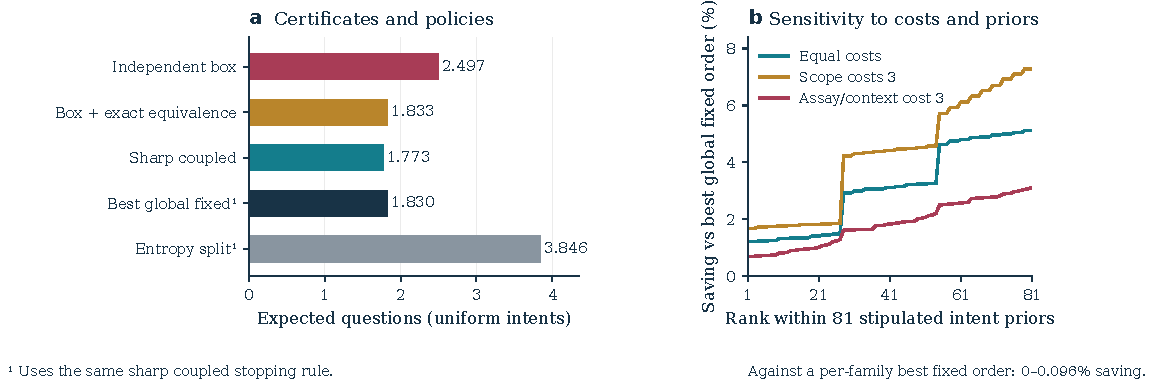
\includegraphics[width=\textwidth]{04_planning.pdf}
\caption{(a) Expected question counts under different certificates and policies. The fixed-order and entropy policies use the same sharp coupled graph; the box comparators optimize their own conservative stopping graphs. (b) The 81 priors in each cost scenario are ranked separately by saving against the hindsight-best global fixed order. These are stipulated sensitivity scenarios, not observed dialogue outcomes. The much stronger per-family fixed comparator nearly eliminates the adaptive advantage.}
\label{fig:planning}
\end{figure*}

\begin{figure*}[t]
\centering
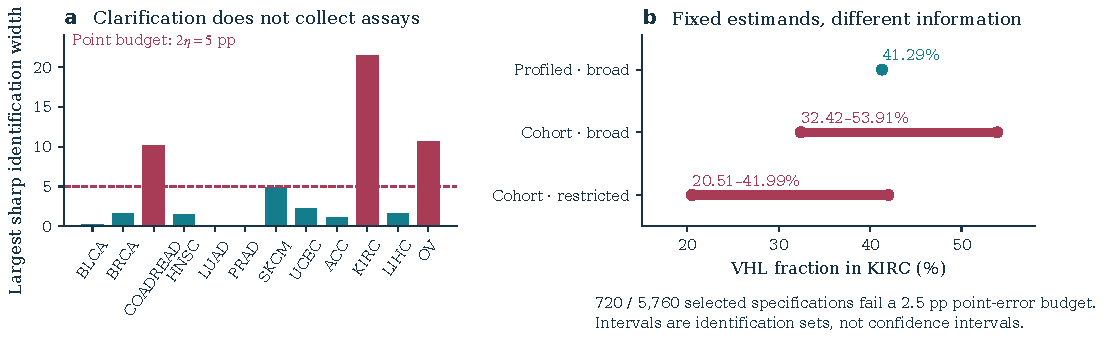
\includegraphics[width=\textwidth]{06_identification.pdf}
\caption{The point guard remains necessary after all intent fields are resolved. (a) Largest sharp interval width by TCGA cohort; the dashed threshold is twice the 2.5 pp minimax point-error budget. (b) KIRC--VHL examples distinguish a fixed profiled fraction from wide cohort-completion intervals. Exactly 720 selected TCGA specifications fail the point budget; this is a registry count, not an observed user failure rate.}
\label{fig:identification}
\end{figure*}

\begin{figure*}[t]
\centering
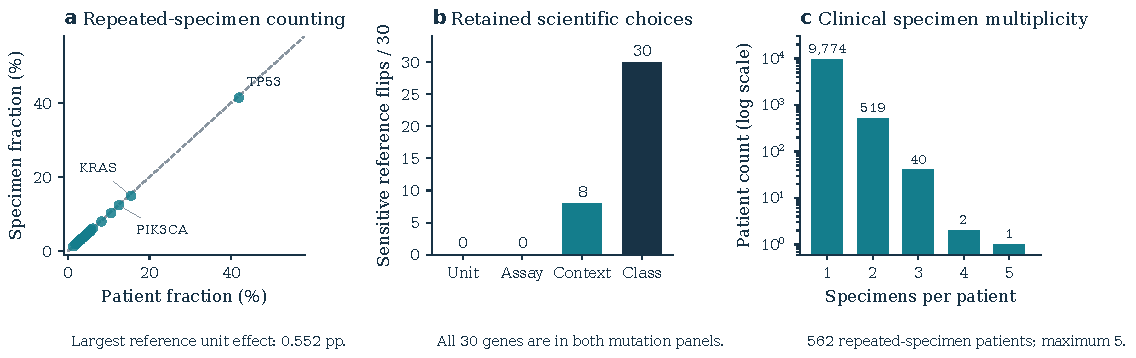
\includegraphics[width=\textwidth]{08_targeted_assay.pdf}
\caption{Separate MSK-IMPACT 2017 stress test, retaining all 30 panel genes. (a) Recorded patient and specimen fractions remain near the diagonal despite repeated specimens. (b) Sensitive reference-axis flips under the primary tolerance. All selected genes are in both source panels, so observed and completion-aware certificates coincide. (c) Patient specimen multiplicity on a logarithmic count axis; 562 patients have two or more specimens. These results challenge counting semantics while exposing the absence of empirical gene-panel missingness in this selected panel.}
\label{fig:msk}
\end{figure*}

\begin{figure*}[t]
\centering
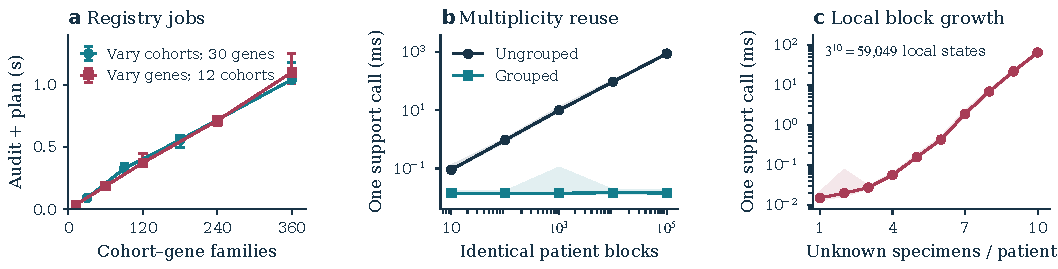
\includegraphics[width=\textwidth]{09_scaling.pdf}
\caption{Measured serial scaling; medians and min--max ranges over five warmed repetitions. (a) Exact certificate-and-planner jobs on prefixes of the frozen cohort/gene lists, after table preparation. (b) Synthetic identical patient tables isolate multiplicity grouping for one integer support. (c) One synthetic repeated-unprofiled patient isolates the retained local exponential cost. Panels time different operations and are not directly comparable. No synthetic rows are new biological evidence.}
\label{fig:scaling}
\end{figure*}

\subsection{Frozen registry and execution checks}
The primary registry uses 12 TCGA PanCancer Atlas cohorts curated in cBioPortal \cite{cerami,gao,hoadley}: BLCA, BRCA, COADREAD, HNSC, LUAD, PRAD, SKCM, UCEC, ACC, KIRC, LIHC, and OV. The unchanged 30-gene panel and every cohort--gene combination yield 360 families, 5,760 specifications, 1,440 reference-axis contrasts, and 43,200 unordered within-family pairs. The snapshot contains 6,210 specimens, 6,204 patients, 5,924 mutation-profiled specimens, and 13,895 panel mutation records. A locally recorded protocol preceded retrieval on 6 October 2026; it is not a public preregistration. The 38 raw JSON responses, normalization, class sets, protocol hashes, and full result tables accompany the paper. Sequential API retrieval is frozen and hashable but not an atomic portal transaction.

SQL \texttt{COUNT(DISTINCT)} and pandas set aggregation independently express the counting queries and agree on positive, denominator, and profiled-unit counts for every specification. They share input normalization and the declared class sets, so agreement alone cannot validate those choices. Sixteen counting contracts and 18 completion/planning contracts pass. Sixty-four small adversarial fixtures enumerate 1,314 global worlds and reproduce every absolute support and relative bound. These fixtures are software verification, not additional biological observations.

TCGA has at most one unprofiled specimen per patient. Consequently its patient contributions are affine in broad/restricted latent indicators. An independently expressed global HiGHS linear program with $0\leq t_s\leq b_s\leq1$ verifies all 43,200 primary paired certificates via integral support objectives: 363 distinct objectives and 172,437 cached repeats. The local-block engine also supports repeated unprofiled specimens and partial patient observation, tested by global enumeration contracts. The TCGA LP check does not establish empirical performance on large repeated-unprofiled blocks.

\subsection{Shared missingness changes the certificate}
Recorded-only execution marks 323/360 families and 23,370/43,200 pairs sensitive. Shared completions mark 356 families and 31,337 pairs. Thus 33 recorded-stable families become completion-sensitive, and 7,967 previously stable pairs can violate tolerance in a feasible shared world (Fig.~\ref{fig:matrix}). This is adversarial possibility, not an estimated probability of an incorrect answer. Low-frequency genes can violate the relative criterion even when absolute changes are small.

Independent interval boxes mark 34,385 pairs sensitive. The 3,048 extra alarms (8.86\% of box alarms) are infeasible paired extremes under the shared model. To distinguish dependence from simple output equivalence, we give a favorable box baseline exact knowledge of all completion-equivalent query functions and merge them. It still marks 31,626 pairs sensitive: 289 alarms remain beyond equivalence, concentrated in OV and SKCM. Fig.~\ref{fig:geometry}c gives a non-equivalent example. These are deterministic full-registry counts; pairwise results within a family are not independent samples and do not justify binomial significance tests.

One-axis sensitivity rises from 428 to 601 of 1,440 contrasts. The complete lattice remains necessary because pairwise extremes can combine multiple field choices. Eleven TCGA cohorts have one specimen per patient; their unit-choice equivalences explain much of the raw-box reduction. We report the equivalence-merged comparator explicitly to avoid crediting all of that reduction to nontrivial dependence.

\subsection{Clarification efficiency and strong baselines}
Under uniform supported intents, the exact planner needs 2.497 questions with independent boxes, 1.833 after equivalence merging, and 1.773 with sharp coupled certificates (Table~\ref{tab:planning}). The reductions are 28.98\% and 3.28\%, respectively. These comparisons preserve the same full completion model; the box's stopping rule is an outer-bound approximation.

\begin{table}[t]
\caption{Uniform, equal-cost clarification over 360 families. All fixed-order and heuristic policies stop using the indicated graph.}
\label{tab:planning}
\centering
\begin{tabular}{lrrr}
\toprule
Certificate & Optimum & Best global & Best per-family\\
 & mean & fixed mean & fixed mean\\
\midrule
Recorded only & 1.149 & 1.238 & 1.149\\
Independent box & 2.497 & 2.554 & 2.498\\
Box + equivalence & 1.833 & 1.890 & 1.834\\
Sharp coupled & 1.773 & 1.830 & 1.773\\
\bottomrule
\end{tabular}
\end{table}

For the sharp graph, the best global fixed order is class, assay, context, then unit. It averages 1.830 questions; the planner saves 3.11\% relative to that comparator. The best \emph{per-family} fixed order and the edge-greedy policy both match the expected optimum, 1.773. Entropy-only splitting averages 3.846; the minimax policy averages 1.818, and both expected and minimax policies can require all four fields. The recorded-only optimum of 1.149 is cheaper but does not certify completion robustness, so it is not an equal-guarantee efficiency comparator.

Across the 243 stipulated prior/cost scenarios, expected-cost savings against the best global fixed order range from 0.695\% to 7.287\%. Against the stronger per-family fixed comparator, savings range from numerical zero to only 0.096\% (Fig.~\ref{fig:planning}). These results support using result-relevant stopping and coupling; they provide little evidence that adaptive branching materially improves a well-configured family-specific order on this registry. All terminal paths satisfy their chosen graph certificate. Across the prespecified 16 tolerance combinations, 343--356 families are sensitive and expected clarification ranges from 1.577 to 1.828 questions.


\subsection{Numerical identification after intent resolution}
With $\eta=2.5$ pp, 720/5,760 fully selected specifications (12.5\%) fail (\ref{eq:guard}), all in COADREAD, KIRC, and OV. They can be semantically unambiguous while lacking enough observations for the point-error budget. KIRC--VHL broad cohort frequency is identified in $[32.42,53.91]\%$, with minimax radius 10.74 pp; its profiled frequency is the fixed recorded fraction 41.29\%. The restricted-class cohort interval is $[20.51,41.99]\%$. These different targets and information states cannot be collapsed into a single mutation ``prevalence'' without qualification (Fig.~\ref{fig:identification}).

A curator can return this interval or acquire evidence. For the fixed KIRC cohort target, measuring 85 of the 110 unknown patients guarantees at most 25 unknown statuses and radius $25/(2\cdot512)=2.44$ pp, regardless of the new outcomes. Alternatively, an externally justified cap of 25 unknown positives would give the conditional interval $[166,191]/512$; a cap of 26 already fails the 2.5 pp budget. These cap calculations are sensitivity illustrations, not claims that the observed frequencies justify a cap. Cross-patient constraints break Cartesian separability and require constrained support optimization; assay sensitivity cannot be inferred from profile membership.


\subsection{Separate clinical targeted-assay stress test}
We retain the same 30 genes in MSK-IMPACT 2017 \cite{zehir}, a mixed-cancer clinical cohort with 10,945 specimens from 10,336 patients, including 562 patients with repeated specimens and up to five specimens per patient. The separate addendum was locally recorded before complete outcome retrieval. DataHub sources are pinned to commit \texttt{dca75cb}; downloaded large-file content hashes and byte counts match its Git LFS pointers. A gene is profiled only if the specimen's declared mutation panel contains it. Primary context uses the source \texttt{SAMPLE\_TYPE=Primary}; one unspecified type remains in all-specimen analyses and is not imputed primary.

Both counting engines agree on all 480 specifications. All selected genes occur in both IMPACT341 and IMPACT410, so this panel has no gene-unprofiled specimens: observed and completion certificates coincide, and every fixed-specification point interval is a singleton. All 30 families are sensitive; reference class flips are sensitive in 30/30, context flips in 8/30, and unit/assay flips in 0/30 (Fig.~\ref{fig:msk}). The largest reference unit effect is 0.552 pp and 4.924\% relative. The optimal, edge-greedy, best global fixed, and best per-family fixed policies all average 1.500 questions; entropy-only splitting requires 4.000. This tests repeated-specimen counting and a targeted-panel adapter, but supplies no additional empirical missing-status or adaptive-planning advantage. It is a distinct clinical cohort in the same curation ecosystem, not an independent portal or a pooled TCGA prevalence estimate.



\subsection{Serial scaling and result-carrying provenance}
A recorded protocol measures five warmed serial repetitions on one AMD EPYC 9V74 worker (Python 3.12.14). Each registry job computes exact graph labels, absolute supports, 40-step relative bounds, and the uniform planner from prepared tables. At 30 genes, increasing cohorts from 1 to 12 takes median 0.089--1.040 s; at 12 cohorts, increasing genes from 1 to 30 takes 0.036--1.099 s. Model preparation takes 20.56 s separately. Timings exclude retrieval, baseline counting, and LP verification (Fig.~\ref{fig:scaling}); the supplement gives full configurations and ranges.

Synthetic workloads isolate computational reuse and its limit. For 100,000 identical one-unknown patient tables, one all-pairs integer support takes 0.898 s ungrouped and 0.0144 ms grouped, with exactly matching outputs. This is an intentionally favorable kernel workload. One patient with 10 unknown specimens requires 59,049 local states and 64.8 ms per support call: local exponential growth remains. Cohort--gene jobs admit independent worker partitions; portal-wide or distributed execution is not measured.

The JSON interface demonstrates three KIRC--VHL outcomes: request clarification, return the cohort interval $[32.42,53.91]\%$, or return the fixed profiled value 41.29\%. Receipts bind requests, model, thresholds, snapshot, implementation, and certificates using SHA-256 and basic PROV-O derivation metadata \cite{prov}. Full replay and nine interface contracts pass. The accompanying offline package includes receipts, timings, and frozen data. This demonstrates a typed integration contract, without an evaluated LLM.



\section{Discussion and Conclusion}
Scientific ambiguity chooses a function; unmeasured specimens determine its shared argument. Marginal intervals discard this dependence and can exaggerate disagreement. Patient-block support preserves it, while the point guard distinguishes semantic stability from sufficient measurement.

Candidate omissions can invalidate semantic coverage. Recorded classes and profile membership do not certify pathogenicity or assay accuracy. Valid external constraints could tighten the broad Cartesian model, while large repeated-unprofiled blocks remain exponential locally. The registry uses one curation ecosystem, TCGA's multiplicity challenge is weak, and stipulated priors/costs do not substitute for researcher interactions. Language accuracy, clinical benefit, and observed user-effort reduction remain unevaluated.

\CLARA{} supplies realizable witnesses, exact cutoff labels, sufficient clarification, and explicit interval answers. Further work should independently annotate interpretations, calibrate interaction costs, and validate additional completion constraints and assay adapters.

\section*{Acknowledgment and AI Disclosure}
OpenAI ChatGPT (Codex) assisted in drafting all manuscript sections, developing mathematical derivations and reproducibility software, and designing all figures. All figures were generated from executed data or the stated completion model, not image synthesis. The authors are responsible for validating the mathematics, code, data use, references, and final submission. Human-participant and language-parser evaluations were not performed.

\begin{thebibliography}{99}
\bibitem{nalir} F. Li and H. V. Jagadish, ``Constructing an interactive natural language interface for relational databases,'' \emph{Proc. VLDB Endow.}, vol. 8, no. 1, pp. 73--84, 2014, doi: 10.14778/2735461.2735468.
\bibitem{ambiqt} A. Bhaskar, T. Tomar, A. Sathe, and S. Sarawagi, ``Benchmarking and improving text-to-SQL generation under ambiguity,'' in \emph{Proc. EMNLP}, 2023, pp. 7053--7074, doi: 10.18653/v1/2023.emnlp-main.436.
\bibitem{saparina} I. Saparina and M. Lapata, ``Disambiguate first, parse later: Generating interpretations for ambiguity resolution in semantic parsing,'' in \emph{Findings of ACL}, 2025, pp. 16825--16839, doi: 10.18653/v1/2025.findings-acl.863.
\bibitem{intentsim} M. J. Q. Zhang and E. Choi, ``Clarify when necessary: Resolving ambiguity through interaction with LMs,'' in \emph{Findings of NAACL}, 2025, pp. 5541--5558, doi: 10.18653/v1/2025.findings-naacl.306.
\bibitem{sage} M. Suri, P. Mathur, N. Lipka, F. Dernoncourt, R. A. Rossi, and D. Manocha, ``Structured uncertainty guided clarification for LLM agents,'' in \emph{Findings of ACL}, 2026, pp. 40811--40838, doi: 10.18653/v1/2026.findings-acl.2028.
\bibitem{incomplete} T. Imieli\'nski and W. Lipski, Jr., ``Incomplete information in relational databases,'' \emph{J. ACM}, vol. 31, no. 4, pp. 761--791, 1984, doi: 10.1145/1634.1886.
\bibitem{dinkelbach} W. Dinkelbach, ``On nonlinear fractional programming,'' \emph{Management Science}, vol. 13, no. 7, pp. 492--498, 1967, doi: 10.1287/mnsc.13.7.492.
\bibitem{garey} M. R. Garey, ``Optimal binary identification procedures,'' \emph{SIAM J. Appl. Math.}, vol. 23, no. 2, pp. 173--186, 1972, doi: 10.1137/0123019.
\bibitem{manski} C. F. Manski, \emph{Partial Identification of Probability Distributions}. New York, NY, USA: Springer, 2003, doi: 10.1007/b97478.
\bibitem{console} M. Console, L. Libkin, and L. Peterfreund, ``Querying incomplete numerical data: Between certain and possible answers,'' in \emph{Proc. PODS}, 2023, pp. 349--358, doi: 10.1145/3584372.3588660.
\bibitem{buneman} P. Buneman, S. Khanna, and W.-C. Tan, ``Why and where: A characterization of data provenance,'' in \emph{Proc. ICDT}, 2001, pp. 316--330, doi: 10.1007/3-540-44503-X\_20.
\bibitem{uldb} O. Benjelloun, A. Das Sarma, A. Halevy, and J. Widom, ``ULDBs: Databases with uncertainty and lineage,'' in \emph{Proc. VLDB}, 2006, pp. 953--964.
\bibitem{green} T. J. Green, G. Karvounarakis, and V. Tannen, ``Provenance semirings,'' in \emph{Proc. PODS}, 2007, pp. 31--40, doi: 10.1145/1265530.1265535.
\bibitem{prov} T. Lebo, S. Sahoo, and D. McGuinness, Eds., ``PROV-O: The PROV ontology,'' W3C Recommendation, Apr. 30, 2013. [Online]. Available: \url{https://www.w3.org/TR/prov-o/}.
\bibitem{cbio_docs} cBioPortal, ``File formats'' and ``Frequently asked questions,'' online documentation. Accessed: Oct. 6, 2026. [Online]. Available: \url{https://docs.cbioportal.org/file-formats/} and \url{https://docs.cbioportal.org/user-guide/faq/}.
\bibitem{cerami} E. Cerami \emph{et al.}, ``The cBio cancer genomics portal: An open platform for exploring multidimensional cancer genomics data,'' \emph{Cancer Discov.}, vol. 2, no. 5, pp. 401--404, 2012, doi: 10.1158/2159-8290.CD-12-0095.
\bibitem{gao} J. Gao \emph{et al.}, ``Integrative analysis of complex cancer genomics and clinical profiles using the cBioPortal,'' \emph{Sci. Signal.}, vol. 6, no. 269, p. pl1, 2013, doi: 10.1126/scisignal.2004088.
\bibitem{hoadley} K. A. Hoadley \emph{et al.}, ``Cell-of-origin patterns dominate the molecular classification of 10,000 tumors from 33 types of cancer,'' \emph{Cell}, vol. 173, no. 2, pp. 291--304.e6, 2018, doi: 10.1016/j.cell.2018.03.022.
\bibitem{zehir} A. Zehir \emph{et al.}, ``Mutational landscape of metastatic cancer revealed from prospective clinical sequencing of 10,000 patients,'' \emph{Nature Medicine}, vol. 23, pp. 703--713, 2017, doi: 10.1038/nm.4333.
\end{thebibliography}

